\PassOptionsToPackage{sols}{handout}
\documentclass[main]{subfiles}
\setcounterrefbeforedot{chapter}{m-ws2-4}
\setcounterrefafterdot{section}{m-ws2-4}
\addtocounter{section}{-1}
\usepackage{solutions}

\begin{document}

\ifSubfilesClassLoaded{%
  \chaptermark{\chaptertwo}
}{}

\section{Trigonometric Functions and Applications} \label{ws2-4}

% \begin{objectives}

% Learning Objectives:

% \begin{itemize}[topsep=0pt,partopsep=0pt,parsep=8pt,itemsep=0pt]

% \item You should understand the definition of $\tan x$ and its unit circle
%   interpretation as the slope of the line between the origin and $P(x)$. 

% \item You should understand the graph of $\tan x$ and its connection with
%   the graphs of $\sin x$ and $\cos x$.

% \item You should be comfortable using both radians and degrees to describe
%   angles.

% \item You should understand the relationship between angles and arc
%   length (by ``arc length,'' we mean the length of an arc of a circle).

% \item You should be able to use symmetry and the unit circle to reason
%   about trigonometric values of related angles.  (For example, you should
%   be able to determine how $\sin(\pi - x)$ relates to $\sin x$.)

% \end{itemize}
% \end{objectives}

\begin{framed}
Here are the six possible ratios of the sides of a right triangle. We've gotten very familiar with sine and cosine, but now it's time to investigate the others: tangent, cosecant, secant, and cotangent.
\begin{minipage}[t]{2in}\vspace{0pt}

\includegraphics[]{tikz/2-2/2-2-right-triangle.pdf}
\end{minipage}
\hspace{12pt}
\begin{minipage}[t]{3in}\vspace{-6pt}
    \[\sin\theta = \dfrac{\text{opp}}{\text{hyp}} \qquad \cos\theta = \dfrac{\text{adj}}{\text{hyp}} \qquad \tan\theta = \dfrac{\text{opp}}{\text{adj}}\]
    \[\csc\theta = \dfrac{\text{hyp}}{\text{opp}} \qquad \sec\theta = \dfrac{\text{hyp}}{\text{adj}} \qquad \cot\theta = \dfrac{\text{adj}}{\text{opp}}\]
\end{minipage}
\vspace{-0.5in}
\end{framed}

\begin{enumerate}

\item 
\begin{problem}
An angle $\theta$ is shown below in standard position on top of the unit circle. It intersects the unit circle at $(x, y)$. Determine the values of the six trigonometric functions in terms of $x$ and $y$.

\begin{minipage}[t]{2.2in}\vspace{0pt}

\includegraphics[]{tikz/2-4/2-4-unit-circle-triangle.pdf}
\end{minipage}
\hspace{12pt}
\begin{minipage}[t]{3.5in}\vspace{0pt}
    \[\sin\theta = \cfitb{0.5in}{y} \qquad \cos\theta = \cfitb{0.5in}{x} \qquad \tan\theta = \cfitb{0.5in}{\frac{y}{x}}\]
    \vspace{36pt}
    \[\csc\theta = \cfitb{0.5in}{\frac{1}{y}} \qquad \sec\theta = \cfitb{0.5in}{\frac{1}{x}} \qquad \cot\theta = \cfitb{0.5in}{\frac{x}{y}}\]
\end{minipage}

\end{problem}

\item 
\begin{problem}
A point $(x,y)$ is at a distance $r$ from the origin and is at an angle $\theta$ from the positive $x$-axis. Determine the values of the six trigonometric functions in terms of $x$, $y$, and $r$.

\begin{minipage}[t]{2.2in}\vspace{0pt}

\includegraphics[]{tikz/2-4/2-4-point.pdf}
\end{minipage}
\hspace{12pt}
\begin{minipage}[t]{3.5in}\vspace{0pt}
    \[\sin\theta = \cfitb{0.5in}{\frac{y}{r}} \qquad \cos\theta = \cfitb{0.5in}{\frac{x}{r}} \qquad \tan\theta = \cfitb{0.5in}{\frac{y}{x}}\]
    \vspace{36pt}
    \[\csc\theta = \cfitb{0.5in}{\frac{r}{y}} \qquad \sec\theta = \cfitb{0.5in}{\frac{r}{x}} \qquad \cot\theta = \cfitb{0.5in}{\frac{x}{y}}\]
\end{minipage}

\end{problem}

\item Notice that, regardless of how far the point is from the origin, $\tan \theta$ is always $\frac{y}{x}$. This has geometric significance: $\tan \theta$ is the slope of the terminal ray when $\theta$ is in standard position.

Using this information, draw an angle $\theta$ in standard position that satisfies
\begin{tasks}(3)
\task $\tan \theta = 5$

\begin{solution}

    \begin{tikzangle}[angle=rad(atan(5))]
    \end{tikzangle}
\end{solution}
\task $\tan \theta = -\frac{1}{2}$

\begin{solution}

    \begin{tikzangle}[angle=rad(atan(-1/2))]
    \end{tikzangle}
\end{solution}
\task $\tan \theta$ is undefined

\begin{solution}

    \begin{tikzangle}[angle=pi/2]
    \end{tikzangle}
\end{solution}
\end{tasks}

\end{enumerate}
\newpage

\begin{enumerate}[resume]
\item 
  \begin{enumerate}
  \item
    \begin{problem}
      Sketch the
      graph of the tangent function. Label the axes with appropriate variables.
      
      \probonly{
      \vspace{12pt}
      
\includegraphics[scale=1.4]{tikz/2-4/2-4-axes.pdf}
      }
    \end{problem}

    \begin{solution}
      Here is the graph:
      \begin{center}
        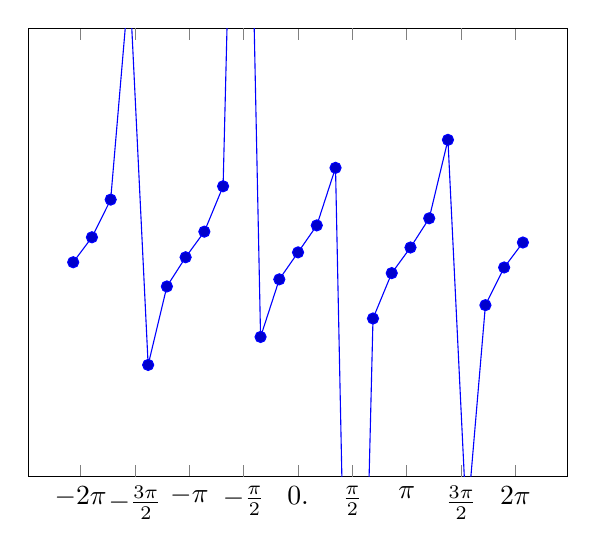
\begin{tikzpicture}
          \begin{axis}[xtick={-6.28319, -3.14159, 0., 3.14159, 6.28319},
            xticklabels={$-2 \pi$, $-\pi$, $0.$, $\pi$, $2 \pi$}, ymin=-5,
            ymax=5, ytick=\empty, extra x ticks={-4.71239, -1.5708, 1.5708,
              4.71239}, extra x tick labels={$-\frac{3 \pi }{2}$,
              $-\frac{\pi }{2}$, $\frac{\pi }{2}$, $\frac{3 \pi }{2}$}]
            \addplot+[domain=-6.5:6.5, restrict y to domain=-20:20]{tan(deg(x))};
          \end{axis}
        \end{tikzpicture}
      \end{center}
    \end{solution}

  \item
    \begin{problem}[\vfill]
    Express $\tan \theta$ in terms of $\sin \theta$ and $\cos \theta$. 
    \end{problem}

    \begin{solution}
      $\tan \theta = \frac{\sin \theta}{\cos \theta}$.
    \end{solution}

  \item

    \note{Students are likely to think that the asymptotes are ``wherever
      the denominator is 0,'' so remind them that it's actually a little
      more nuanced than that.  You might have them look at a simple
      example like $\frac{x - 5}{x - 5}$.} 

    \begin{problem}[\stretch{1}]
      Where are the vertical asymptotes of the graph? Why are there vertical asymptotes there?      
    \end{problem}

    \begin{solution}
      The asymptotes of $\tan x$ occur at $\pm \frac{\pi}{2}, \pm \frac{3
        \pi}{2}, \ldots$.  In other words, they happen at $x =
      \frac{\pi}{2} + n \pi$, where $n$ is any integer.

      This makes sense with the fact that $\tan x = \frac{\sin x}{\cos
        x}$: at $\frac{\pi}{2} + n \pi$, $\cos x = 0$ and $\sin x \neq
      0$. 
    \end{solution}

  \item

    \note{Similarly, students are likely to think that the zeros are
      ``wherever the numerator is 0,'' but $\frac{x - 5}{x - 5}$ is a
      counterexample again.}

    \begin{problem}[\stretch{1}]
      Where are the horizontal intercepts of the graph?  Why are there intercepts at these values?
    \end{problem}

    \begin{solution}
      The zeros of $\tan x$ are $0, \pm \pi, \pm 2 \pi, \ldots$.  In other
      words, they are $n \pi$ where $n$ is an integer.

      This makes sense with the fact that $\tan x = \frac{\sin x}{\cos
        x}$: at integer multiples of $\pi$, $\sin x = 0$ and $\cos x \neq
      0$, so $\frac{\sin x}{\cos x} = 0$.
    \end{solution}

  \item
    \begin{problem}
      What is the period of the tangent function? How does this relate to the unit circle?
    \end{problem}
    \pspace{\vfill}
    
    \begin{solution}
      We can see from the graph that the period is $\pi$. 
    \end{solution}

  \item
    Evaluate the following limits.

    \probonly{}
      \begin{enumerate}
      \item
        \begin{problem}
          $\displaystyle \lim_{\theta \to (\pi/2)^-} \tan \theta$
        \end{problem}
        \pspace{\stretch{0.5}}

        \begin{solution}
          From the graph, we see that this limit is $\boxed{\infty}$.
          (This means that the limit does not exist, but saying the limit
          is $\infty$ is more informative than simply saying the limit
          does not exist.)
        \end{solution}

      \item
        \begin{problem}
          $\displaystyle \lim_{\theta \to (\pi/2)^+} \tan \theta$
        \end{problem}
        \pspace{\stretch{0.5}}

        \begin{solution}
          From the graph, we see that this limit is $\boxed{-\infty}$. 
        \end{solution}

      \item

        \note{They have never seen this type of behavior before.  You may
          want to also ask them about something like $\displaystyle
          \lim_{\theta \to \infty} \sin \theta$ or $\displaystyle \lim_{\theta \to
            -\infty} \cos \theta$.
            
            
            Matt note - this can be a good plug for the idea of a limit. I often informally discuss limits with Math M students as the answer to the question "what does it look like the function is doing as we..." If this answer isn't clear, we might have more work to do, or if it's clear that there isn't a specific answer (such as the case of $\tan x$, then the limit doesn't exist (even though it isn't $\infty$ or $-\infty$!)}

            

        \begin{problem}
          $\displaystyle \lim_{\theta \to \infty} \tan \theta$
        \end{problem}
        \pspace{\stretch{0.5}}

        \begin{solution}
          From the graph, we see that, as $\theta$ increases without bound,
          $\tan \theta$ does not head toward any particular value.  Therefore,
          this limit \fbox{does not exist}.
        \end{solution}

      \end{enumerate}

  \end{enumerate}
\end{enumerate}

\pspace{\newpage}

\begin{enumerate}[resume]
\item 
\begin{problem}
    Express $\sec \theta$, $\csc \theta$, and $\cot \theta$ in terms of $\sin \theta$ and $\cos \theta$.
\end{problem}
\pspace{\vfill}

\begin{solution}
Using our answers to \#1, we can determine that
    \begin{itemize}
        \item $\sec\theta=\frac{1}{\cos\theta}$
        \item $\csc\theta=\frac{1}{\sin\theta}$
        \item $\cot\theta=\frac{\cos\theta}{\sin\theta}$
    \end{itemize}
\end{solution}

\item  Give an exact value for each expression, if it is defined.

\begin{solution}
    We can use our knowledge of the unit circle and the relationships we just found in \#5 to find these values.
\end{solution}

\begin{tasks}[after-item-skip=48pt, after-skip=48pt](4)
    \task $\sec \frac{\pi}{4}\solonly{=\sqrt{2}}$
    \task $\tan \frac{3\pi}{4}\solonly{=-1}$
    \task $\csc \frac{5\pi}{4}\solonly{=-\sqrt{2}}$
    \task $\cot \frac{7\pi}{4}\solonly{=-1}$

    \task $\tan \frac{7\pi}{3}\solonly{=\sqrt{3}}$
    \task $\csc\!\left(-\frac{5\pi}{6}\right)\solonly{=-2}$
    \task $\cot\!\left(-\frac{2\pi}{3}\right)\solonly{=\frac{\sqrt{3}}{3}}$
    \task $\sec\frac{13\pi}{6}\solonly{=\frac{2\sqrt{3}}{3}}$


    \task $\cot\!\left(-\frac{3\pi}{2}\right)\solonly{=0}$
    \task $\csc 4\pi\solonly{\text{ is undefined}}$
    \task $\sec \frac{11\pi}{2}\solonly{\text{ is undefined}}$
    \task $\tan\!\left(-\frac{\pi}{2}\right)\solonly{\text{ is undefined}}$

    
\end{tasks}

  % \probonly{}
  %   \begin{enumerate}    
  %   \item
  %     \begin{problem}
  %       $\csc( - \frac{5\pi}{6})$
  %     \end{problem}

  %     \begin{solution}
  %       $\csc \left( - \frac{5 \pi}{6} \right)$ is defined to be
  %       $\frac{1}{\sin \left( - \frac{5 \pi}{6} \right)}$, so let's first
  %       find $\sin \left( - \frac{5 \pi}{6} \right)$.  As usual, we'll
  %       first draw the angle in standard position (in red below), and then
  %       we can use the reference triangle (in green):
  %       \begin{center}
  %         \begin{tikzangle}[angle=-5*pi/6, triangle=true]          
  %         \end{tikzangle}          
  %       \end{center}
  %       The reference angle is $\frac{\pi}{6}$, so the vertical side has
  %       length $\frac{1}{2}$.  Therefore, $\sin \left( - \frac{5 \pi}{6}
  %       \right) = - \frac{1}{2}$ and $\csc \left( - \frac{5 \pi}{6}
  %       \right) = \boxed{-2}$.
  %     \end{solution}

  %   \item
  %     \begin{problem}
  %       $\displaystyle \cot \left ( - \frac{3\pi}{2} \right )$
  %     \end{problem}

  %     \begin{solution}
  %       $\cot \left( - \frac{3 \pi}{2} \right)$ is defined to be
  %       $\frac{\cos \left( - \frac{3 \pi}{2} \right)}{\sin \left( -
  %           \frac{3 \pi}{2} \right)}$, so let's first find $\cos \left( -
  %         \frac{3 \pi}{2} \right)$ and $\sin \left( - \frac{3 \pi}{2}
  %       \right)$.  As usual, we draw the angle in standard position:
  %       \begin{center}
  %         \begin{tikzangle}[angle=-3*pi/2]
  %         \end{tikzangle}          
  %       \end{center}
  %       We don't need a reference triangle here because we can tell the
  %       coordinates of the point $P\left( - \frac{3 \pi}{2} \right)$
  %       already: the point is $(0, 1)$.  So, $\cos \left( - \frac{3
  %           \pi}{2} \right) = 0$, $\sin \left( - \frac{3 \pi}{2} \right) =
  %       1$, and $\cot \left( - \frac{3 \pi}{2} \right) = \boxed{0}$.
  %     \end{solution}

  %   \item
  %     \begin{problem}
  %       $\displaystyle \sec \left( \frac{13 \pi}{6} \right)$
  %     \end{problem}

  %     \begin{solution}
  %       $\sec \left( \frac{13 \pi}{6} \right)$ is defined to be
  %       $\frac{1}{\cos \left( \frac{13 \pi}{6} \right)}$, so let's first
  %       find $\cos \left( \frac{13 \pi}{6} \right)$.  Here is the angle
  %       $\frac{13 \pi}{6}$ in standard position:
  %       \begin{center}
  %         \begin{tikzangle}[angle=13*pi/6, triangle=true,
  %           refangledistance=12pt]            
  %         \end{tikzangle}
  %       \end{center}
  %       The reference angle is $\frac{\pi}{6}$, so the horizontal side of
  %       the reference triangle has length $\frac{\sqrt{3}}{2}$.
  %       Therefore, $\cos \left( \frac{13 \pi}{6} \right) =
  %       \frac{\sqrt{3}}{2}$ and $\sec \left( \frac{13 \pi}{6} \right) = 
  %       \boxed{\frac{2}{\sqrt{3}}}$.

  %       (Alternatively, you might have just noticed $\frac{13 \pi}{6}$ is
  %       $2\pi$ more than $\frac{\pi}{6}$; since $\cos$ repeats every $2
  %       \pi$, that means $\cos \left( \frac{13 \pi}{6} \right) = \cos
  %       \left( \frac{\pi}{6} \right)$.)
  %     \end{solution}

  %   \end{enumerate}

\item
\begin{enumerate}
    \item
    \begin{problem}
    On the axes below, sketch the graph of sine.

    \probonly{
    
\includegraphics[scale=1.4]{tikz/2-4/2-4-axes.pdf}
    }
    \end{problem}

\begin{solution} The graph of sine is shown in red.
      \begin{center}
        \begin{tikzpicture}
          \begin{axis}[xtick={-4.71239, -1.5708, 1.5708, 4.71239},
            xticklabels={$-\frac{3 \pi }{2}$, $-\frac{\pi }{2}$,
              $\frac{\pi }{2}$, $\frac{3 \pi }{2}$}, ytick={-1, 1}, extra
            x ticks={-6.28319, -3.14159, 0.01, 3.14159, 6.28319}, extra x
            tick labels={$-2 \pi$, $-\pi$,, $\pi$, $2 \pi$}, ymin=-4,
            ymax=4, xmin=-6.6, xmax=6.6, extra x tick style={grid=major,
              grid style={dashed, thick, blue}}, xlabel=$\theta$]
              \addplot[domain=-6.5:6.5, red]{sin(deg(x)};
            \addplot+[domain=-6.5:6.5, restrict y to domain=-15:15, blue]{1/sin(deg(x))};
            \addplot[closed] coordinates {(-4.71, 1) (-1.57, -1) (1.57,1) (4.71, -1)};
          \end{axis}
        \end{tikzpicture}
      \end{center}
    \end{solution}   

    \item
    \begin{problem}
        If $\sin\theta=1$, what is $\csc\theta$? Show this on the graph.
    \end{problem}
    \pspace{\stretch{0.5}}

    \begin{solution}
        If $\sin\theta=1$, then $\csc\theta=\frac{1}{\sin\theta}=1$.
    \end{solution}

    \item
    \begin{problem}
        If $\sin\theta=0$, what is $\csc\theta$? Show this on the graph.
    \end{problem}
    \pspace{\stretch{0.5}}

    \begin{solution}
        If $\sin\theta=0$, then $\csc\theta=\frac{1}{\sin\theta}$ is undefined. so there are vertical asymptotes on the graph of cosecant at $\theta = 0, \pm \pi, \pm
      2\pi$. 
    \end{solution}

    \item
    \begin{problem}
        Sketch the graph of cosecant on the same axes.
    \end{problem}

    \begin{solution}
        See the blue graph above.
    \end{solution}
\end{enumerate}

  \end{enumerate}

\pspace{\newpage}



\textbf{Key Idea}: Trigonometry can be used to solve geometric problems involving lengths and angles.

\begin{enumerate}[resume]

\item 
  \note{On this problem and the next, be sure that students are drawing
    good pictures. Deciphering the language in these problems to get a
    good sense of things is frequently the hardest part.}

  \begin{problem}[\stretch{0.5}]
    You're interested in knowing the height of a tall tree.  You position
    yourself so that your line of sight to the top of the tree makes a
    $60^{\circ}$ angle with the horizontal.  You measure the distance from
    where you stand to the base of the tree to be 45 feet.  How tall is
    the tree, if your eyes are five feet above the ground?
  \end{problem}

  \begin{solution}
    Here's a diagram of the situation (not to scale):
    \begin{center}
      \begin{tikzpicture}[x=0.35cm, y=0.35cm]
        \coordinate (tree) at (10, 7); %
        \coordinate (eyes) at (0, 2); %
        \draw (eyes) -- (tree) -- (tree |- 0, 0); %
        \draw[decorate, decoration={brace}] ($(tree) + (2pt, 0)$) --
        node[right, xshift=2pt]{tree} ($(tree |- 0, 0) + (2pt, 0)$); %
        \filldraw (eyes) circle(1.5pt) node[left]{your eyes}; %
        \draw ($(eyes) + (8pt, 0)$) arc[radius=8pt, start angle=0, end
        angle={atan(1/2)}] node[anchor=185, xshift=4pt]{$60^\circ$}; %
        \draw[dashed] (eyes) -- (tree |- eyes); %
        \draw[dashed] (eyes) -- node[left]{5} (eyes |- 0, 0); %
        \draw (-1, 0) -- (11, 0) node[right]{ground}; %
        \draw[|-|] ($(eyes |- 0, 0) - (0, 1em)$) -- node[fill=white] {45}
        ($(tree |- 0, 0) - (0, 1em)$); %
      \end{tikzpicture}
    \end{center}
    We have a right triangle in our picture, so we can use trigonometry:
    $\tan 60^\circ = \frac{\text{length of vertical side of
        triangle}}{45}$, so the vertical side is $45 \tan (60^\circ) = 45
    \cdot \tan \left( \frac{\pi}{3} \right) = 45 \sqrt{3}$.  The height of
    the entire tree is the length of this vertical side plus 5, or
    \fbox{$45 \sqrt{3} + 5$ ft}.
  \end{solution}
  
\item 

  We are standing on flat ground in Monument Valley trying to
  estimate the height of the edifices.  We have surveying equipment and
  take all of our measurements from a height of 5 feet.  We find the angle
  of elevation to the top of one structure is $23^{\circ}$. We move 500
  feet closer to the structure and find that the angle of elevation is now
  $29^{\circ}$.

  
\includegraphics{images/go20p06.pdf}

  \emph{This problem is an example of \textbf{triangulation}: by
      taking angle measurements from two different viewpoints, we can
      determine both the size and distance of an object.  This principle
      has a huge variety of applications.  For example, in medical
      imaging, triangulation is used to determine the size and location of
      tumors in a patient's body so that targeted treatment can be
      delivered.}

  \begin{enumerate}
  \item
    \begin{problem}[\stretch{1}]
      How tall is the structure?  Give an exact answer, as well as a
      decimal approximation.
    \end{problem}

    \begin{solution}
      We're looking for the height of the structure; let's call that $H$.
      If use $h$ to represent length CD in the picture below, then
      $H=h+5$.
      There are two right triangles in the picture that we can take
      advantage of, ACD and BCD. We know that angle CAD is \ang{23} and
      angle CBD is \ang{29}. Since the angle measurements are taken
      $500$ feet apart, length AB is $500$ feet.
      Let's name the other horizontal distance that might be
      useful; let $x$ be the length of BD.
      \begin{center}
        \begin{tikzpicture}[x=1.5cm, y=1.5cm]
          \coordinate (ground) at (0, -0.4); %
          \coordinate (A) at (0, 0); %
          \coordinate (B) at (1, 0); %
          \coordinate (C) at (4, 2); %
          \coordinate (D) at (4, 0);
          \draw[very thick] (A) node[below left] {$A$} -- 
          (C) node[above] {$C$} -- (D) node[below left] {$D$}; %
          \draw[very thick] (B) node[below left] {$B$} -- (C) -- (D); %
          \draw[very thick, dashed] (A) -- (D);
          \draw[decorate, decoration={brace, mirror}] 
          ($(A |- ground) - (0,2pt)$) -- node[below, yshift=-2pt]
          {$500$ feet} ($(B |- ground) - (0, 2pt)$); %
          \draw[decorate, decoration={brace, mirror}] 
          ($(B |- ground) - (0,2pt)$) -- node[below, yshift=-2pt]{$x$} 
          ($(C |- ground) - (0,2pt)$); %
          \draw (C |- A) -- (C); %
          \draw pic[draw=black, "\ang{23}", angle radius = 20, angle eccentricity = 1.5] {angle=D--A--C};
          \draw pic[draw=black, "\ang{29}", angle radius = 20, angle eccentricity = 1.5] {angle=D--B--C};
          \draw (A) -- (ground) -- (C |- ground) -- (C |-
          A); %
          \draw (B) -- (B |- ground); %
          \draw[decorate, decoration={brace}] ($(C)+(2pt,0)$) -- 
          node[right,xshift=2pt]{$h$} ($(D)+(2pt,0)$);
          \draw[decorate, decoration={brace}] ($(D)+(2pt,0)$) -- 
          node[right,xshift=2pt]{$5$ feet} ($(D |- ground)+(2pt,0)$);
        \end{tikzpicture}
      \end{center}
      From triangle BCD, we can relate our variables with the equation
      \[ \tan 29^\circ = \frac{h}{x}.\]
      From triangle ACD,
      \[ \tan 23^\circ = \frac{h}{x + 500}.\]
      We can rewrite the equations as
      \begin{align}
        x \tan 29^\circ &= h \\
        (x + 500) \tan 23^\circ &= h
        \end{align}
      There are many ways to solve this system of equations. One way
      would be to substitute $x \tan\ang{29}$ for $h$ in equation (2),
      \begin{align*}
        x \tan \ang{29}  &= (x + 500) \tan \ang{23}.
        \intertext{We can then solve this for $x$:}
        x \tan 29^\circ &= x \tan 23^\circ + 500 \tan 23^\circ \\
        x (\tan 29^\circ - \tan 23^\circ) &= 500 \tan 23^\circ \\
        x &= \frac{500 \tan 23^\circ}{\tan 29^\circ - \tan 23^\circ}.
      \end{align*}
      Finally, we can plug this back into either equation
      (1) or equation
      (2) to solve for $h$; equation
      (1) looks simpler.  From equation
      (1), $h = x \tan 29^\circ =
        \frac{500 \tan 23^\circ \tan 29^\circ}{\tan 29^\circ - \tan
          23^\circ} \text{ feet}$, so we can conclude that
          $H = h+5 = \boxed{\frac{500 \tan 23^\circ \tan 29^\circ}{\tan 29^\circ - \tan
          23^\circ}+5 \text{ feet}}$ or about \fbox{$911$ feet.}
    \end{solution}

  \item
    \begin{problem}[\stretch{0.25}]
      When we make the second measurement, how far away are we from the
      structure we're measuring?
    \end{problem}

    \begin{solution}
      We found this in part (a): $x=\boxed{\frac{500 \tan
          23^\circ}{\tan 29^\circ - \tan 23^\circ} \text{ feet}}$
          or about \fbox{$1635$ feet.}
    \end{solution}

  \end{enumerate}

\end{enumerate}

\end{document}